\documentclass[journal,transmag]{IEEEtran}

% ..........................................................................
% Packages, configuration settings, and macro definitions.

\usepackage[pdftex]{graphicx}
\graphicspath{figures}
\DeclareGraphicsExtensions{.pdf,.jpeg,.png}

\usepackage[pdftex,rgb,dvipsnames,svgnames,hyperref,table]{xcolor}

\usepackage[pdftex,breaklinks=true,colorlinks=true,
    bookmarks=false,pdfhighlight=/O,
    urlcolor=DarkBlue,citecolor=DarkRed,linkcolor=DarkBlue]{hyperref}

\usepackage[cmex10]{amsmath}
\interdisplaylinepenalty=2500

\usepackage{amssymb}
\usepackage{amsfonts}
\usepackage{multicol}
\usepackage{multirow}
\usepackage{enumitem}
\usepackage{accsupp}
\usepackage{array}
\usepackage[caption=false,font=footnotesize]{subfig}
\usepackage{booktabs}
\usepackage{xspace}
\usepackage{soul}
\usepackage{url}
\usepackage{hyphenat}
\usepackage[english]{babel}
\usepackage[square,numbers,sort&compress]{natbib}
\usepackage{booktabs}

% Correct bad hyphenation here
\hyphenation{}

\newcommand{\email}[1]{\href{mailto:#1}{#1}}

\usepackage{pdfcomment}
\newcommand{\comment}[3]{\pdfmarkupcomment[markup=Highlight,color=yellow,author={#2}]{#1}{#3}}

\usepackage{tabularx}
% ..........................................................................
% Body.

\begin{document}
\nocite{IEEEBSTcontrol}
\markboth{IEEE Transactions on Biomedical Engineering}{Standards for whole-cell modeling}

\title{Toward standards for tomorrow's whole-cell models}

\author{
    Dagmar Waltemath$^{*,+}$,
    Jonathan R. Karr$^+$, 
    Frank T. Bergmann,
    Vijayalakshmi Chelliah,
    Michael Hucka,\\
   Marcus Krantz,
    Wolfram Liebermeister,
   Pedro Mendes,
    Chris J. Myers,~\IEEEmembership{Senior~Member,~IEEE,}
    Pinar Pir,\\
    %%%%%%%%%%%%%%%%%%%
    Begum Alaybeyoglu,
    Naveen K Aranganathan,
    Arne T. Bittig,
    Paulo E. Pinto Burke, 
    Yin Hoon Chew,
    Rafael S. Costa,\\
    Joseph Cursons, 
    Tobias Czauderna,
%    Muhammad Haseeb,
    Denis Kazakiewic, 
    Ilya Kiselev,
    Vincent Knight-Schrijver,\\
    Christian Kn\"{u}pfer,
    Matthias K\"{o}nig,
    Nikita Mandrik,
    J. Kyle Medley,
    Bertrand Moreau, \\
    Sucheendra K. Palaniappan,
   Daniel Priego-Espinosa, 
    Martin Scharm,
    Mahesh Sharma,
    Kieran Smallbone,\\
    Je-Hoon Song,
    Tom Theile,
    Milenko Tokic, 
    Namrata Tomar, 
    Jannis Uhlendorf, 
    Thawfeek M Varusai,\\
    Florian Wendland, 
    Markus Wolfien,
    James T. Yurkovich,
    Yan Zhu, 
    Argyris Zardilis, 
    Anna Zhukova, and
    Falk Schreiber$^+$\\
	
    \thanks{
        Manuscript received XXX XX, 2015; revised XXX XX, 201X; accepted XXX XX, 201X. Date of publication XXX XX, 201X; date of current version XXX XX, 201X.
        This work was supported in part by the Volkswagen Foundation (Grant to D. W. and F. S.) and the James S. McDonnell Foundation (Postdoctoral Fellowship Award in Studying Complex Systems to J. R. K.).
        \textit{Asterisk indicates corresponding author. Plus indicates these authors contributed equally to this work.}
    }
    \thanks{$^*$D. Waltemath, A. T. Bittig, M. Scharm, T. Theile, F. Wendland and M. Wolfien are with the Institute of Computer Science, University of Rostock, 18051 Rostock, Germany (e-mail: \email{dagmar.waltemath@uni-rostock.de}; \email{arne.bittig@uni-rostock.de}; \email{martin.scharm@uni-rostock.de}; \email{tom.theile@uni-rostock.de}; \email{florian.wendland@uni-rostock.de}; \email{markus.wolfien@uni-rostock.de}).}    
    \thanks{J.~R. Karr is with the Department of Genetics \& Genomic Sciences, Icahn School of Medicine at Mount Sinai, New York, NY 10029, USA (e-mail: \email{karr@mssm.edu}).}
    \thanks{C.~J. Myers is with the Department of Electrical and Computer Engineering, University of Utah, Salt Lake City, Utah 84112, USA (e-mail: \email{myers@ece.utah.edu}).}
    \thanks{M. Hucka is with the Department of Computing and Mathematical Sciences, California Institute of Technology, Pasadena, CA 91125, USA (e-mail: \email{mhucka@caltech.edu}).}
    \thanks{F.~T. Bergmann is with BioQuant, University of Heidelberg, 69120 Heidelberg, Germany (e-mail: \email{fbergman@caltech.edu}).} 
    \thanks{N.~K. Aranganathan and V. Chelliah are with the European Bioinformatics Institute (EMBL-EBI), European Molecular Biology Laboratory, Cambridge CB10 1SD, UK (e-mail: \email{navyeinstein1991@gmail.com, viji@ebi.ac.uk}).}   
    \thanks{M. Krantz and J. Uhlendorf are with the Department of Biology, Humboldt University of Berlin, 10115 Berlin, Germany (e-mail: \email{marcus.krantz@biologie.hu-berlin.de}; \email{jannis.uhlendorf@hu-berlin.de}).}
    \thanks{W. Liebermeister and M. K\"{o}nig are with the Institute of Biochemistry, University Medicine Charit\'{e} Berlin, 10117 Berlin, Germany (e-mail: \email{wolfram.liebermeister@gmail.com}; \email{matthias.koenig@charite.de}).}
    \thanks{P. Mendes is with the Manchester Institute of Biotechnology and the School of Computer Science, University of Manchester, Manchester M1 7DN, UK and also with the Center for Quantitative Medicine and the Department of Cell Biology, University of Connecticut Health Center, Farmington, CT 06030, USA (e-mail: \email{pedro.mendes@manchester.ac.uk}).}
    \thanks{P. Pir and V. Knight-Schrijver are with the Babraham Institute, Cambridge CB22 3AT, UK (e-mail: \email{pinar.pir@babraham.ac.uk}).}
    \thanks{B. Alaybeyoglu is with the Department of Chemical Engineering, Bo\v{g}azi\c{c}i University, Bebek 34342, Turkey (e-mail: \email{begum.alaybeyoglu@boun.edu.tr}).}
    \thanks{P.~E. Pinto Burke is with the Institute of Science and Technology, Federal University of S\~{a}o Paulo, Brazil.}
    \thanks{Y.~H. Chew is with the Centre for Synthetic and Systems Biology, University of Edinburgh, Edinburgh EH9 3BF, UK (e-mail: \email{yinhoon.chew@ed.ac.uk}).}
    \thanks{R.~S. Costa is with the Centre of Intelligent Systems-IDMEC, Instituto Superior T{\'e}cnico, University of Lisbon, 1049-001 Lisboa, Portugal (e-mail: \email{rafael.s.costa@tecnico.ulisboa.pt}).}
    \thanks{J. Cursons is with the Department of Biomedical Engineering, School of Engineering, University of Melbourne, Parkville, VIC 3010, Australia (e-mail: \email{joseph.cursons@unimelb.edu.au}).}
    \thanks{T. Czauderna and F. Schreiber are with the Faculty of Information Technology, Monash University, Clayton, VIC 3800, Australia and also with the Institute of Computer Science, Martin Luther University Halle-Wittenberg, 06108 Halle, Germany (e-mail: \email{tobias.czauderna@monash.edu}; \email{falk.schreiber@monash.edu}).}
%    \thanks{M. Haseeb is with the Department of Bioinformatics, Mohammad Ali Jinnah University, Islamabad, Pakistan.}
    \thanks{D. Kazakiewic is with the Center for Statistics, Universiteit Hasselt, Hasselt BE3500, Belgium, and also with the Center for Innovative Research, Medical University of Bia\l{}ystok, Bia\l{}ystok 15-089, Poland (e-mail: \email{dzianis.kazakevich@uhasselt.be}).}
    \thanks{I. Kiselev is with the Design Technological Institute of Digital Techniques, Siberian Branch of the Russian Academy of Sciences, Novosibirsk 630090, Russia.}
    \thanks{C. Kn\"{u}pfer is with the Institut f\"ur Informatik, University of Jena, 07743 Jena, Germany (e-mail: \email{christian.knuepfer@uni-jena.de}).}
    \thanks{N. Mandrik is with the Sobolev Institute of Mathematics, Siberian Branch of the Russian Academy of Sciences, Novosibirsk 630090, Russia (e-mail: \email{manikitos@gmail.com}).}
    \thanks{J.~K. Medley is with the Department of Bioengineering, University of Washington, Seattle, WA 98195, USA (e-mail: \email{medleyj@uw.edu}).}
    \thanks{B. Moreau is with the CoSMo Company, Lyon, France (e-mail: \email{bertrand.moreau@thecosmocompany.com}).}
    \thanks{S.~K. Palaniappan is with the Rennes - Bretagne Atlantique Research Centre, Institute for Research in Computer Science and Automation, 35042 Rennes Cedex, France.}
    \thanks{D.~Priego-Espinosa is with the Instituto de Ciencias F{\'i}sicas, Universidad Nacional Aut{\'o}noma de M{\'e}xico, M{\'e}xico.}
    \thanks{M. Sharma is with the Department of Pharmacoinformatics, National Institute of Pharmaceutical Education and Research, Punjab 160062, India.}
    \thanks{K. Smallbone is with the Manchester Centre for Integrative Systems Biology, University of Manchester, Manchester M1 7DN, UK (e-mail: \email{kieran.smallbone@manchester.ac.uk}).}
    \thanks{J.-H. Song is with the Department of Bio and Brain Engineering, Korea Advanced Institute of Science and Technology, Daejeon 305-701, Republic of Korea (e-mail: \email{song.je-hoon@kaist.ac.kr}).}
    \thanks{M. Tokic is with the Laboratory of Computational Systems Biotechnology (LCSB), Swiss Federal Institute of Technology (EPFL), CH-1015 Lausanne, Switzerland and with the Swiss Institute of Bioinformatics (SIB), CH-1015 Switzerland (e-mail: \email{milenko.tokic@epfl.ch}).}
    \thanks{N. Tomar is with the Department of Dermatology, University Medicine, Friedrich-Alexander University of Erlangen-N\"urnberg, 91052 Erlangen, Germany.}
   \thanks{T.~M. Varusai is with the Department of Systems Biology Ireland, University College Dublin, Belfield, Dublin 4, Ireland (e-mail: \email{thawfeek.varusai@ucdconnect.ie}).}
    \thanks{J. T. Yurkovich is with the Department of Bioengineering, University of California, San Diego, La Jolla, CA 92093, USA (e-mail: \email{jyurkovich@ucsd.edu}).}
    \thanks{Y. Zhu is with Monash Institute of Pharmaceutical Sciences, Monash University, Parkville, VIC 3052, Australia.}
    \thanks{A. Zardilis is with the Centre for Synthetic and Systems Biology, University of Edinburgh, UK.} 
    \thanks{A. Zhukova is with the Institut de Biochimie et G\'en\'etique Cellulaires, National Center for Scientific Research, and also with the University of Bordeaux, France, 33077 Bordeaux Cedex, France (e-mail: \email{zhutchok@gmail.com}).}
    \thanks{Digital Object Identifier 10.1109/TBME.XXXX.XXXXXXX}
}

\maketitle

\begin{abstract}
Whole-cell modeling is a promising tool for biological research, bioengineering, and medicine. 
However, substantial work remains to create complete, accurate, and reproducible models.
Among the advances needed are a strong theoretical understanding of multi-algorithm modeling, standardized modeling languages, and an efficient general-purpose simulator.
We organized the 2015 Whole-Cell Modeling Summer School to teach whole-cell modeling, as well as to evaluate the need for new modeling standards and tools by encoding a recently published whole-cell model in SBML.
We describe several standards extensions, software tools, and databases which are needed to facilitate reproducible whole-cell modeling, including a graphical model editor, a multi-algorithm simulator, and several SBGN extensions.
Together these new standard extensions and software tools could accelerate whole-cell modeling.
\end{abstract}

\begin{IEEEkeywords}
Whole-cell modeling, Systems biology, Computational biology, Simulation, Standards, Education
\end{IEEEkeywords}

\IEEEpeerreviewmaketitle

\section{Introduction}

\IEEEPARstart{O}{ver} the past twenty years, computational modeling has become an essential and powerful tool for biological research, bioengineering, and medicine to analyze high-throughput molecular measurements and understand the molecular details of complex biological systems. Computational modeling has been used to identify new metabolic genes~\cite{Reed2006}, to engineer metabolic pathways in bacteria~\cite{Lee2012}, and to identify potential new antimicrobial drug targets~\cite{Lee2009}.
Computational models also have the potential to enable bioengineers to design new microorganisms for industrial applications such as chemical synthesis, biofuel production, and waste decontamination, as well as to enable clinicians to tailor therapy to individual patients. Realizing this potential requires more comprehensive and accurate computational models that are capable of predicting cellular behavior from genotype. Realizing this potential also requires improved simulation tools, as well as standardized tools for storing and exchanging models, simulation experiments, and visualizations~\cite{Macklin2014,Karr2015,Karr2015b,hucka2015promoting,Klipp07,path2models2013}.

Recently, researchers at Stanford University developed the first whole-cell model of the gram-positive bacterium \textit{Mycoplasma genitalium}~\cite{Karr2012}. The model represents the life cycle of a single Mycoplasma cell including the copy number dynamics of each metabolite, RNA, and protein species and accounts for every known gene function. The model is composed of 28 submodels, each of which is implemented using different mathematical formalisms including \emph{ordinary differential equations} (ODEs), \emph{flux balance analysis} (FBA), and \emph{Boolean rules} (BRs), and trained using different experimental data. 
The model is implemented in MATLAB, is available open-source under the MIT license~\cite{wholeCell}, and is extensively documented. This has enabled other researchers to use the model to conduct \textit{in silico} experiments~\cite{Sanghvi2013, Purcell2013, Kazakiewicz2015}. 

Despite extensive documentation, this whole-cell model software is difficult to use. The software is large, complex, and time-consuming to learn. The software also cannot easily be reused to simulate other models because many of the model details are intertwined with the software. In addition, many academic researchers and many software developers cannot use the model software because MATLAB is proprietary and expensive. Compared to other languages with larger development communities such as Python, MATLAB has also few packages and development tools. In particular, MATLAB has limited support for object-oriented programming. Furthermore, the model software is not optimally efficient because MATLAB is just-in-time compiled and dynamically typed.

Covert and colleagues developed the WholeCellKB~\cite{Karr2013}, WholeCellSimDB~\cite{Karr2014}, and WholeCellViz~\cite{Lee2013} software tools to provide user-friendly interfaces to their modeling software. However, significant domain expertise is still required to use their modeling software, particularly to construct new models. Alternative approaches are needed to enable more researchers to develop and simulate their own whole-cell models. Software-independent standards and other open-source software tools have the potential to enable researchers to develop such models more quickly, to explore them more deeply, and to evaluate them more rigorously. Furthermore, standards would make whole-cell models more reusable and comparable, as well as more searchable and retrievable through model repositories such as BioModels~\cite{juty2015biomodels,chelliah2015biomodels}.

Several software-agnostic systems biology standards have already been developed by the \emph{COmputational Modeling in BIology NEtwork} (COMBINE)~\cite{le2011meeting}, including the \emph{Systems Biology Markup Language} (SBML)~\cite{hucka2003}, the \emph{Cell Markup Language} (CellML)~\cite{hedley_2001b}, the \emph{Simulation Experiment Description Markup Language} (SED-ML)~\cite{sedml2011}, and the \emph{Systems Biology Graphical Notation} (SBGN)~\cite{LeNovereHMMSS09}. SBML and CellML are languages for representing mathematical models. CellML focuses on modularly encoding mathematical models, while SBML focuses on describing biological processes. Both support several modeling formalisms including ODEs and FBA. SED-ML is a language for describing computational experiments, including the simulation algorithm and parameter values. SED-ML enables scientists to reproduce simulations. SBGN is a visual notation for describing biological processes. To date, none of these open standards have been used with models as complex as the \textit{M. genitalium} model.

We organized the 2015 Whole-Cell Modeling Summer School to train students in whole-cell modeling, as well as to evaluate the need for new standards and tools for whole-cell modeling. The majority of the school focused on encoding the \textit{M. genitalium} model using SBML, visualizing it with SBGN, and simulating it with SED-ML. This was both a learning exercise, as well as a tool for evaluating standard representations capabilities for encoding whole-cell models. The ultimate goal of the school was to encode an open-source whole-cell model in SBML, visualize the model using SBGN, simulate the model using open-source software, and use the model to conduct \textit{in silico} experiments encoded in SED-ML. We chose to focus the course on SBML because there was insufficient time to evaluate both SBML and CellML.

Here, we describe the summer school, outline our progress encoding the \textit{M. genitalium} model using standards, and describe several standard extensions and software tools that we believe are needed to support efficient whole-cell modeling.

\section{The 2015 Whole-Cell Modeling Summer School}
We organized the summer school to teach students how to build and encode models using COMBINE standards by encoding the \textit{M. genitalium} model using software-independent, standard representation formats.

\subsection{Organization}
The Whole-Cell Modeling Summer School was held March 9-13, 2015 at the University of Rostock, Germany. The school was organized by Dagmar Waltemath and Falk Schreiber and supported by the Volkswagen Foundation. The school included 45 students, nine instructors, and two organizers.

The school began with two introductory lectures on modeling and modeling standards. Jonathan Karr from the Icahn School of Medicine at Mount Sinai, USA, presented an overview of whole-cell and multi-algorithm modeling. Michael Hucka from the California Institute of Technology, USA, presented an overview of the SBML, SED-ML, and SBGN standards; open-source software tools that support these standards; and the COMBINE initiative. We also organized three discussions on model composition, particle-based state representation, and stochastic modeling. 

The majority of the school was devoted to hands-on learning about whole-cell modeling and the COMBINE standards by encoding the \textit{M. genitalium} model in SBML, creating visualizations using SBGN, and defining simulations using SED-ML. The 28 sub-models were divided among nine groups of four to five students and one instructor.
Each day concluded with brief progress reports from each group to exchange ideas and facilitate discussion.
We also organized a poster session and several social activities to encourage students to network.

\subsection{Educational outcome}
Most students reported gaining knowledge of whole-cell modeling, increased appreciation for reproducibility, and increased understanding of the SBML, SED-ML, and SBGN standards. Many students also reported learning about open-source software tools relevant to their own research.

In addition, many of the students reported that the school expanded their network. The school introduced several students to other workshops and job opportunities.

\subsection{Lessons learned for organizing research-based schools}
We learned several valuable lessons about how to best organize a research-based school. First, we learned that research-based schools should have clear background knowledge expectations and learning objectives and have well-planned learning exercises. This helps students make informed decisions about whether to participate in the school, know how to prepare for the school, and learn efficiently.
Second, we found that students greatly enjoy learning through open research problems rather than through prescribed training exercises. This challenges students and engages them in research. This also helps students build practical skills that complement their undergraduate training.
Third, we found that open-ended project-based schools require a high teacher-to-student ratio, a flexible schedule, and multidisciplinary project teams. A high teacher to student ratio allows students to get feedback and iterate through potential solutions quickly. A flexible schedule enables impromptu lectures and discussions. Multidisciplinary teams enable students to work through difficult problems by drawing on perspectives from multiple fields. 

\section{Toward an SBML-encoded whole-cell model}
In addition to training young researchers, the second goal of the school was to encode the \textit{M. genitalium} whole-cell model in SBML. To achieve this goal, most of the course was devoted to active learning sessions in which students were challenged to encode submodels of the \textit{M. genitalium} in SBML, integrate submodels into a single model, and simulate models using SED-ML. During these sessions, the students and instructors were divided into nine groups. Eight of the groups were tasked with encoding one or more submodels. The ninth group was tasked with developing a standards-compliant scheme to integrate the submodels into a single model. In addition, three instructors helped all of the groups annotate and visualize their submodels and one instructor helped all of the groups encode their submodels in SBML. Table~SI lists the nine groups and all of the students and instructors. 

\subsection{Submodel encoding}
The eight submodel encoding groups pursued various strategies to encode submodels in SBML. Several of the groups encoded submodels by first reading the submodel documentation, then drawing pathway diagrams using software tools such as CellDesigner~\cite{funahashi2008celldesigner} and VANTED~\cite{Rohn2012}, and finally writing scripts to generate SBML models from their diagrams using libSBML~\cite{bornstein_2008}. Other groups used modeling software tools such as Antimony~\cite{Smith2009}, BioUML~\cite{Kolpakov2006}, COBRApy~\cite{ebrahim2013cobrapy}, COPASI~\cite{Mendes2009}, iBioSim~\cite{Madsen2012}, and libRoadRunner~\cite{Somogyi17062015} to encode submodels based on their documentation. A few of the groups encoded submodels by converting the MATLAB code to SBML. These groups then generated SBGN diagrams from their SBML to better understand their submodels.

The groups encountered several challenges to encoding the submodels in SBML. First, understanding the submodels was time-consuming because the documentation only summarizes the submodels, the connection between the submodels and the associated pathway/genome database is unclear, and many of the submodels details are implemented directly in the MATLAB code. Fortunately, one of the principal authors of the \textit{M. genitalium} model participated in the school.

A second challenge to encoding the submodels was to encode serially-executed MATLAB submodels in SBML, because SBML does not explicitly represent sequential operations. Most of the groups decided to tackle this problem by formalizing MATLAB submodels as discrete stochastic models and simulating them using the Gillespie stochastic simulation algorithm~\cite{gillespie1977}. One drawback of this approach is that it required assigning kinetics that are not present in the original MATLAB submodels due to insufficient kinetic data.

A third challenge to encoding the submodels was to encode the randomized algorithms used by the MATLAB submodels in SBML. For example, the MATLAB translation submodel includes a randomized algorithm that assigns amino acids to individual polypeptides. This algorithm is not equivalent to the Gillespie algorithm and cannot easily be encoded in SBML because plain SBML does not support random number generation. Most of the groups also solved this problem by formalizing submodels as stochastic models.

To encode many of the submodels in SBML, the groups also had to either enumerate the particle-based state representation used by the MATLAB submodels, or approximate the MATLAB submodels. The translation group chose to approximate their submodel by eliminating the internal dynamics of the polymerization of each polypeptide. Consequently, their submodel does not track the progress of individual ribosomes or account for base-specific translation rates. The replication, replication initiation, transcription, and transcriptional regulation groups, chose to enumerate the chromosome representation used by the MATLAB model by creating Boolean indicator variables to represent the existence and protein-binding status of each base. This enumerated representation requires millions of variables. Consequently, the corresponding SBML files are computationally expensive to parse and simulate. Enumerating the rules that govern the joint values of the enumerated variables, such as the rules that represent the steric effects of DNA-bound proteins by preventing proteins from binding neighboring bases, is also impractical. Furthermore, editing this enumerated representation is difficult because thousands of variables and rules must be edited rather than a small number of variable and rule patterns.

The lack of SBML simulator support for arrays was another challenge to encoding submodels in SBML. All of the groups overcame the lack of array support by enumerating individual array elements and all matrix algebra computations. This created verbose SBML files that are difficult to interpret, maintain, and edit. Enumerating the matrix algebra computations also increases the computational cost of simulation.

Combined, we found it difficult to encode most of the MATLAB submodels in SBML. As discussed below, future progress in whole-cell modeling would be facilitated by expanded support for the SBML Multistate and Multicomponent Species~\cite{SBMLMulti} and SBML Arrays~\cite{SBMLArrays} packages.

\subsection{Model integration}
The integration group was responsible for assembling the submodels into a single model. This included devising a scheme for representing global state variables, defining the interfaces exposed by the submodels to the global state variables, and developing a method to manage concurrent writing of shared state variables by multiple submodels. The integration group defined the global state variables as the union of all state variables shared by at least two submodels rather than by explicitly defining a set of global state variables as done by the original MATLAB-based simulation. The advantages of this approach are that submodel developers are not also required to develop global state variables and that it minimizes the number of global state variables. The disadvantages of this approach are that the total set of variables is less transparent and that it requires users to learn all of the submodels and their naming conventions to analyze model simulations.

The integration group standardized the submodel interfaces by defining a variable naming convention. This convention makes it clear how multiple local submodel variables map onto the same global variable. The integration group used the same variable names as those used by the MATLAB implementation. Matrix and particle-based variables were enumerated by creating multiple variables differentiated by the suffixes.

The primary challenge faced by the integration group was managing concurrent editing of state variables by multiple submodels. The group explored several potential solutions. First, they explored sequentially simulating the submodels and updating the global state variables. This avoids needing to merge variable changes. However, under this approach, submodels are simulated with different variable values within each time step. Consequently, simulation predictions are sensitive to the submodel execution order. 

The integration group also explored several more complex solutions that would enable submodels to be simulated with the same variable values within each time step. These strategies included reducing the submodel integration time step so that submodels do not request conflicting variable changes; dividing each of the shared state variables into multiple, independent sub-variables for each submodel, simulating the submodels, and merging the sub-variables to update global values; and using semaphores to manage concurrent variable editing whereby at each time step submodels request sets of atomic state changes and a controller decides which change sets are accepted. Each of these strategies has advantages and disadvantages. The first strategy is simple to understand and implement, but is computationally expensive. The second strategy is simple to implement and computationally efficient for independent variables, but is complex for coupled variables such as those that represent the chromosome protein occupancy. The third strategy is complex, but is more general than the second strategy and more computationally efficient than the first. Ultimately, we concluded that a combination of these strategies will be needed to efficiently manage concurrent writing of different types of shared variables. The integration group implemented their strategies using either SBML, SED-ML, or hierarchical SBML models. The integration group tested their strategies using iBioSim because iBioSim is one of the few simulators that supports model composition.

Another challenge to integrating the submodels was the lack of a multi-algorithm simulator. The integration group plans to overcome this limitation by adding support for multi-algorithm simulation to iBioSim.

\begin{figure*}[bt!]
\centering
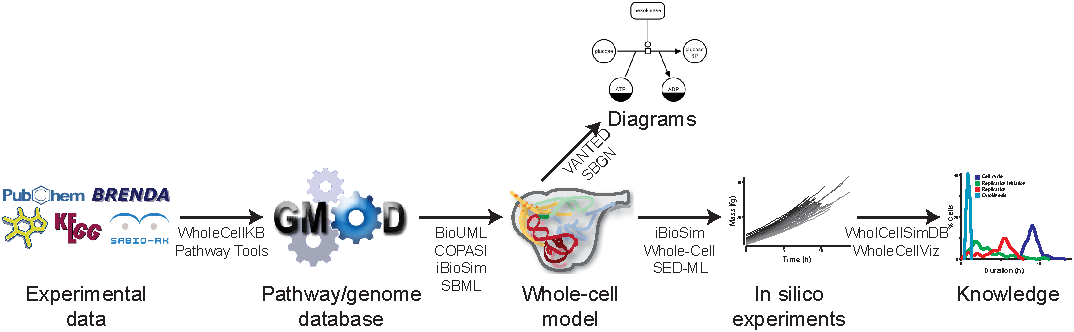
\includegraphics[width=\textwidth]{figure1/figure1.pdf}
\caption{\label{fig:1} Whole-cell modeling pipeline. First, researchers will assemble experimental data into pathway/genome databases. Second, researchers will use pathway/genome databases to construct submodels. Third, researchers will use multi-algorithm simulators to conduct \textit{in silico} experiments. Lastly, researchers will analyze in silico experiments to learn new biology.}
\end{figure*}

\subsection{Annotation, documentation, and visualization}
The documentation group was responsible for annotating the model.
The goal was to annotate every model entity with a cross reference to an external database such as ChEBI~\cite{Hastings2013}, as in the case of small molecules, and/or in terms of other model entities, as in the case of chemical reactions.
The group wrote scripts to search molecular biology databases for every entity contained in the \textit{M. genitalium} model.
The main problem faced by the documentation group was that many model entities are not currently represented by any molecular biology database.
This shortcoming can easily be overcome by proposing new ontology terms to the databases.
This problem highlights the need to expand the molecular biology databases to aggregate data on more biological molecules and interactions. 

The documentation group also helped the other groups visualize submodels by providing advice on SBGN and diagramming tools such as VANTED~\cite{Rohn2012}.
The main visualization problem encountered by the documentation group was that whole-cell models require large diagrams that must be manually arranged to produce intuitive visualizations.

\subsection{Progress}
We produced preliminary SBML and SBGN versions of most of the \textit{M. genitalium} submodels and finished SBML and SBGN versions for the cytokinesis submodel. Significant work remains to finish encoding the model. We must finish encoding the submodels, expand software tools such as iBioSim to support multi-algorithm modeling, rigorously test the SBML model by reproducing all of the MATLAB model tests, and thoroughly diagram and document the SBML model.

\subsection{Future steps}
We hope to finish encoding the \textit{M. genitalium} submodels in SBML and integrating the SBML-encoded submodels into a single model that can be simulated by open-source software tools such as BioUML, COPASI, iBioSim, and libRoadRunner. Several students and instructors have continued to work and meet online. Many also plan to participate in a second meeting in October, 2015, that will be held at the University of Utah, USA, immediately prior to the 2015 COMBINE Forum.

Going forward, we hope to publish SBML-encoded versions of each of the \textit{M. genitalium} submodels to BioModels, along with SED-ML tests, SBGN diagrams, and textual documentations. This would make the submodels searchable, retrievable, and reusable by other scientists. We believe this would be a valuable community resource. It would demonstrate how to build a whole-cell model and enable other researchers to build upon the \textit{M. genitalium} submodels.

\section{Toward SBML-, SED-ML-, and SBGN-based standards for whole-cell modeling}
The school was the first attempt to encode a whole-cell model using open standards. It is thus unsurprising that it revealed limitations with currently-available formats, but it also generated ideas for how existing standards and tools can be expanded to better support large, heterogeneous models.

\subsection{Standard extensions}
Several enhancements to simulation software tools and databases are needed to facilitate whole-cell modeling. First, more SBML simulators must support multi-algorithm simulations. This will require research to determine the best way to integrate heterogeneous submodels, including rigorously evaluating the schemes proposed by the integration group. Significant effort will also be needed to develop an efficient, parallelized, multi-algorithm simulator.

Second, more SBML simulators must implement the SBML Multistate and Multicomponent Species package to support hybrid population/particle-based state representation such as that used by BioNetGen \cite{Hlavacek2006, Hogg2014} and NFSim \cite{Sneddon2011}. This would enable more succinct model descriptions, making models much easier to understand, edit, and expand. For example, translation could be described using a single reaction pattern and arrays of mRNA-specific translation initiation rates and codon-specific elongation rates rather than by enumerating each reaction. By separating mathematical descriptions from quantitative parameter values, reaction patterns would also make the connection between dynamical models and the experimental data used to inform their parameters more transparent. Implementing the SBML Multistate and Multicomponent Species package would also enable modelers to efficiently simulate models with large, combinatorial state spaces.

New user-friendly graphical editors must also be developed to enable researchers to easily build SBML files with these new features. These graphical editors must also allow researchers to transparently map model parameters onto experimental data organized in pathway/genome databases.

In addition, our molecular biology databases such as ChEBI must be expanded to enable researchers to concretely define whole-cell models in terms of external entities. 

SBGN must also be expanded in several ways. SBGN must be expanded to support hybrid diagrams which contain Process Descriptions, Entity Relationships, and Activity Flow maps. The SBGN viewers must also be expanded to provide layout algorithms suitable for large visualizations and automatically display diagrams at multiple levels of granularity using contextual zooming and model reduction. 

Together, these software, database, and SBGN expansions would enable more researchers to more easily build, manage, simulate, and reproduce whole-cell models and simulations. These new standards and tools would also enable researchers to build more comprehensive and more accurate models. Ultimately, this would enable whole-cell modeling to support bioengineering and personalized medicine.

\subsection{The whole-cell modeling pipeline}
We anticipate that such expanded standards and tools will enable a four step approach to whole-cell model-driven discovery (Fig.~\ref{fig:1}). First, researchers will assemble experimental data from numerous sources including databases such as SABIO-RK~\cite{Wittig2012} and UniProt~\cite{UniProt2015} into pathway/genome databases using software tools such as Pathway Tools~\cite{Karp2010} and WholeCellKB. Second, researchers will use pathway/genome databases and graphical modeling tools such as BioUML, COPASI, and iBioSim to build submodels and encode them using transparent languages such as SBML. Third, multi-algorithm simulators will be used to conduct \textit{in silico} experiments. Lastly, software tools such as WholeCellSimDB and WholeCellViz will be used to discover new biology through exploring, visualizing, and analyzing in silico experiments.

\section{Conclusion}
The 2015 Whole-Cell Modeling Summer School provided 45 young scientists training in whole-cell and multi-algorithm modeling by encoding the \textit{M. genitalium} whole-cell model in SBML. Additional courses are needed to provide students with deeper theoretical training in dynamical modeling, multi-algorithm modeling, model reduction, and parameter estimation, as well as practical training in model construction including data curation, model building, numerical optimization, model testing, and model analysis.

The summer school also made valuable strides toward encoding the \textit{M. genitalium} whole-cell model using SBML for simulation by open-source software. We developed preliminary SBML versions of all of the submodels of the \textit{M. genitalium} model. We have continued to encode the \textit{M. genitalium} model since the school. Ultimately, we hope to publish an SBML-encoded version of the model to BioModels. 

In addition, the summer school generated clear goals for expanding the existing SBML software tools to support whole-cell modeling. The SBML simulators must be expanded to support all of the Hierarchical Model Composition, Multistate and Multicomponent Species, Arrays, and Flux Balance Constraints packages to efficiently simulate whole-cell models. Furthermore, the school unified modelers, software developers, and standards developers to develop standardized, open-source tools for whole-cell and other large models.

New parameter estimation, model testing, and visual analysis tools must also be developed to enable researchers to effectively use SBML-encoded whole-cell models for research. In addition, our molecular biology databases must be expanded to facilitate whole-cell model annotation. Furthermore, SBGN and the SBGN viewers must be expanded to support hybrid diagrams, automatic graph layout, automatic graph reduction, and contextual zooming. CellML should also be rigorously evaluated as another potential whole-cell modeling standard.

In summary, we believe that whole-cell modeling has the potential to be an important tool for biological discovery, bioengineering, and medicine. Achieving this potential requires new simulation software for simulating whole-cell models. In turn, this requires expanding the whole-cell modeling field including training additional young researchers.

\ifCLASSOPTIONcaptionsoff
  \newpage
\fi

\bibliographystyle{IEEEtran}
\bibliography{IEEEabrv,report}

% biography section
% 
% If you have an EPS/PDF photo (graphicx package needed) extra braces are needed around the contents of the optional argument to biography to prevent
% the LaTeX parser from getting confused when it sees the complicated \includegraphics command within an optional argument. (You could create
% your own custom macro containing the \includegraphics command to make things simpler here.)

\begin{IEEEbiography}[{\includegraphics[width=3.45in,keepaspectratio]{photos/group.jpg}}]{}
~\\
~\\
~\\
~\\
~\\
~\\
~\\
~\\
~\\
~\\
~\\
\textbf{2015 Whole-Cell Modeling Summer School} included the 56 participants listed in Table~SI.
\end{IEEEbiography}


% You can push biographies down or up by placing a \vfill before or after them. The appropriate
% use of \vfill depends on what kind of text is on the last page and whether or not the columns are being equalized.

\vfill

% Can be used to pull up biographies so that the bottom of the last one is flush with the other column.
%\enlargethispage{-5in}

% ..........................................................................
% End.

\clearpage
\setcounter{table}{0}
\renewcommand{\thetable}{S\Roman{table}}

\begin{table*}[ht!]
\caption{2015 Whole-Cell Modeling Summer School participants.}
\begin{tabularx}{\textwidth}{llX}
\toprule
\textbf{Group}           & \textbf{Participant}            & \textbf{Affiliation}\\
\midrule
Cytokinesis               & Naveen Kumar Aranganathan        & European Bioinformatics Institute , UK\\
                          & Daniel Priego-Espinosa           & National Autonomous University of Mexico, Mexico\\
                          & Ilya Kiselev                     & Siberian Branch of the Russian Academy of Sciences Novosibirsk, Russia\\
                          & Wolfram Liebermeister            & Charit\'e Medical University of Berlin, Germany\\
                          & Yan Zhu                          & Monash University, Australia\\
\midrule
DNA repair                & Arne Bittig                      & University of Rostock, Germany\\
                          & Vijayalakshmi Chelliah           & European Bioinformatics Institute, UK\\
                          & Audald Lloret-Vilas              & European Bioinformatics Institute, UK\\
                          & Mahesh Sharma                    & National Institute of Pharmaceutical Education and Research, India\\
                          & Namrata Tomar                    & Friedrich-Alexander University of Erlangen-N\"urnberg, Germany\\
\midrule
Metabolism                & Kambiz Baghalian                 & University of Oxford, UK\\
                          & Frank T. Bergmann                & University of Heidelberg, Germany\\
                          & Rafael Sousa Costa               & University of Lisbon, Portugal\\
                          & Matthias K\"onig                 & Charit\'e Medical University of Berlin, Germany\\
                          & Kieran Smallbone                 & University of Manchester, UK\\
                          & Milenko Tokic                    & Swiss Federal Institute of Technology in Lausanne, Switzerland\\
\midrule
Protein                   & Begum Alaybeyoglu                & Bo\v{g}azi\c{c}i University, Turkey\\
                          & Matteo Cantarelli                & OpenWorm, UK\\
                          & Yin Hoon Chew                    & University of Edinburgh, UK\\
                          & Marcus Krantz                    & Humboldt University of Berlin, Germany\\
                          & Daewon Lee                       & Korea Advanced Institute of Science and Technology, Republic of Korea\\
\midrule
Replication               & Vincent Knight-Schrijver         & Babraham Institute, UK\\
                          & Je-Hoon Song                     & Korea Advanced Institute of Science and Technology, Republic of Korea\\
                          & Jannis Uhlendorf                 & Humboldt University of Berlin, Germany\\
                          & Dagmar Waltemath                 & University of Rostock, Germany\\
                          & James T. Yurkovich                  & University of California, San Diego, USA\\
                          & Anna Zhukova                     & National Center for Scientific Research and University of Bordeaux, France\\
\midrule
Replication initiation    & Harold Gomez                     & Boston University, USA\\
                          & Jens Hahn                        & Humboldt University of Berlin, Germany\\
                          & Michael Hucka                    & California Institute of Technology, USA\\
                          & Nikita Mandrik                   & Siberian Branch of the Russian Academy of Sciences Novosibirsk, Russia\\
                          & Martin Scharm                    & University of Rostock, Germany\\
                          & Florian Wendland                 & University of Rostock, Germany\\
\midrule
RNA                       & Tuure Hameri                     & Swiss Federal Institute of Technology in Lausanne, Switzerland\\
                          & J. Kyle Medley                   & University of Washington, USA\\
                          & Sucheendra Kumar Palaniappan     & Institute for Research in Computer Science and Automation, France\\
                          & Pinar Pir                        & Babraham Institute, UK\\
                          & Natalie Stanford                 & University of Manchester, UK\\
                          & Markus Wolfien                   & University of Rostock, Germany\\
\midrule
Translation               & Joseph Cursons                   & University of Melbourne, Australia\\
                          & Muhammad Haseeb                  & Mohammad Ali Jinnah University, Pakistan\\
                          & Daniel Hernandez                 & Swiss Federal Institute of Technology in Lausanne, Switzerland\\
                          & Denis Kazakiewicz                & University of Hasselt, Belgium and Medical University of Bia\l{}ystok, Poland\\
                          & Pedro Mendes                     & University of Manchester, UK\\
                          & Hojjat Naderi Meshkin            & Academic Center for Education, Culture and Research, Iran\\
\midrule
Integration               & Paulo Eduardo Pinto Burke        & Federal University of S\~ao Paulo, Brazil\\
                          & Tobias Czauderna                 & Monash University, Australia\\
                          & Bertrand Moreau                  & CoSMo Company, France\\
                          & Chris J. Myers                   & University of Utah, USA\\
                          & Thawfeek Mohamed Varusai         & University College Dublin, Ireland\\
                          & Argyris Zardilis                 & University of Edinburgh, UK\\
\midrule
Annotation, documentation & Christian Kn\"upfer              & University of Jena, Germany\\
and visualization         & Falk Schreiber                   & Monash University, Australia\\
                          & Tom Theile                       & University of Rostock, Germany\\
\midrule
Modeling instructor       & Jonathan R. Karr                 & Icahn School of Medicine at Mount Sinai, USA\\
\bottomrule
\end{tabularx}
\end{table*}

\end{document}
